%!TEX root = report.tex

\section{Data Description}
\label{Sec:ProblemData}

Yi and Eisenstein have provided the data used in [1].
The data consists of a collection of tweets as well as some network information on Twitter.

\subsection{Corpus}
The corpus contains a collection of samples (tweets). 
For each data sample, we have one tweet ID, one user ID, a sentiment label (positive, neutral, negative), and the tweet content itself. For example, the following are two examples of our data samples.
\begin{verbatim}
261140278944088066	17572408	negative	@USER may i have an industrial revolution ...
237571817550786563	727519172	neutral	@USER i told you shane would get his 5th-star ...
\end{verbatim}

The size of the corpus is the following:
\begin{figure}[hbt]
\centering
  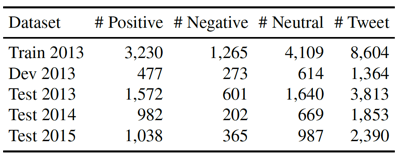
\includegraphics{Picture1.png}
  \caption{dataset description}
\end{figure}


\subsection{Network}
We have contacted Yi, one of the author of [1], to obtain the three social networks he used in the paper,
i.e.,
FOLLOWER, MENTION and RETWEET network. The construction of each network is seen in [1].
Each network is an edge list of form:
\begin{verbatim}
73225701 8161232
95679562 87818409
...
\end{verbatim}
On each line, the two numbers are user IDs, indicating that there is an edge (direct connection) between the two nodes.
The first and second are two user IDs which are consistent with the above twitter data. These two user IDs indicate these two users are connected in the network. 

{
Three social network structures were constructed in [1]. As described in the original paper:
\begin{description}
	\item 

~~~~~\emph{
We construct three author social networks based on the follow, mention, and retweet relations between the 7,438 authors in the training dataset,
which we refer as FOLLOWER, MENTION and RETWEET. Specifically, we use the Twitter API to crawl the friends of the SemEval users (individuals
that they follow) and the most recent 3,200 tweets in their timelines. The mention and retweet links are then extracted from the tweet text and metadata.
We treat all social networks as undirected graphs, where two users are socially connected if there exists at least one social relation between them.}
\end{description}
}
